\documentclass[11pt,a4paper]{jsarticle}
%
\usepackage{amsmath,amssymb}
\usepackage{bm}
\usepackage[dvipdfmx]{graphicx}
\usepackage{ascmac}
\usepackage{titlesec}
\usepackage{otf}
\usepackage{amsthm}
\usepackage{physics}
\usepackage{booktabs}
%
\setlength{\textwidth}{\fullwidth}
\setlength{\textheight}{39\baselineskip}
\addtolength{\textheight}{\topskip}
%\setlength{\voffset}{-0.1in}
\setlength{\topmargin}{0pt}
\setlength{\headheight}{0pt}
\setlength{\headsep}{0pt}

% \renewcommand{\thesection}{演習問題\arabic{section}}
% \titleformat*{\section}{\normalsize\bfseries}
% \titleformat*{\subsection}{\normalsize\bfseries}

\newtheorem{problem}{演習問題}
\newtheorem{answer}{解答}
\renewcommand{\theanswer}{}
\newcommand{\N}{\mathcal{N}}
%
%\newcommand{\divergence}{\mathrm{div}\,}  %ダイバージェンス
%\newcommand{\grad}{\mathrm{grad}\,}  %グラディエント
%\newcommand{\rot}{\mathrm{rot}\,}  %ローテーション
\newcommand{\Zahlen}{\mathbb{Z}}
\newcommand{\const}{\mathrm{const}}
\newcommand{\laplace}{\mathcal{L}}

\begin{document}

\begin{center}
  {\Large\bfseries \TeX 演習問題} % title
\end{center}
\begin{flushright}
  {\large 43M21224 諏訪 棟植} % 学生番号と氏名と氏名を書き換えてください
\end{flushright}

% 提出するファイル名は,practice_YourName.pdfにしてください.
% 例:practice_SuwaMuneue.pdf
%
% 大文字のデルタや円周率パイなど,不明なギリシャ文字はググってください.
%
% 図は,パワポなどで作成した後,PDFファイルで保存したうえで,
% pdfcropコマンドでトリミングしてください.
% なお,図の問題は,pdfファイルの図を挿入することを目的として出題しているため,
% 図自体は適当でかまいません.

\section{数学}

\subsection{フーリエ級数展開}

% ここから編集してください

$f(x)$のフーリエ級数展開を\eqref{fourier-series}に示す.
\begin{align}\label{fourier-series}
  f(x)\sim\frac{a_0}{2}+\sum_{n=1}^\infty\left(a_n\cos \omega_nx+b_n\sin \omega_nx\right)
\end{align}
ただし,$a_n,b_n$は,
\begin{align*}
  a_n & =\frac{2}{T}\int_0^T f(x)\cos\omega_nx dx,~(n=0,1,2,3,\cdots) \\
  b_n & =\frac{2}{T}\int_0^T f(x)\sin\omega_nx dx,~(n=1,2,3,\cdots)
\end{align*}
である.

\subsection{フーリエ変換表}

フーリエ変換表を表\ref{tab:fourier-transform}に示す.ただし,
\begin{align*}
  f(0^+)=\lim_{t\to 0}f(t)
\end{align*}
である.

\begin{table}[hbt]
  \centering
  \caption{フーリエ変換表}
  \label{tab:fourier-transform}
  \begin{tabular}{c|c}
    $f(t)$                & $F(s)$                        \\ \hline
    $f^\prime(t)$         & $sF(s)-f(0^+)$                \\
    $f^{\prime\prime}(t)$ & $s^2F(s)-sf(0)-f^\prime(0^+)$ \\
    $t^ne^{-at}$          & $n!/(s+a)^{n+1}$              \\
  \end{tabular}
\end{table}

\subsection{余因子行列}

余因子行列$\tilde{A}$は,余因子$A_{ij}:=(-1)^{i+j}\Delta_{ij}$を用いると,
\begin{align*}
  \tilde{A}=
  \begin{bmatrix}
    A_{11} & A_{21} & \cdots & A_{n1} \\
    A_{12} & A_{22} & \cdots & A_{n2} \\
    \vdots & \vdots & \ddots & \vdots \\
    A_{1n} & A_{2n} & \cdots & A_{nn} \\
  \end{bmatrix}
\end{align*}
と表される.

\section{物理}

\subsection{ラミの定理}

図\ref{fig:lami-s-theorem}に示すように,点Oに作用している3力$F_1,F_2,F_3$が釣り合っているとき,
\begin{align*}
  \frac{F_1}{\sin(\pi-\theta_1)}=\frac{F_2}{\sin(\pi-\theta_2)}=\frac{F_3}{\sin(\pi-\theta_3)}
\end{align*}
となる.

\begin{figure}[hbtp]\centering
  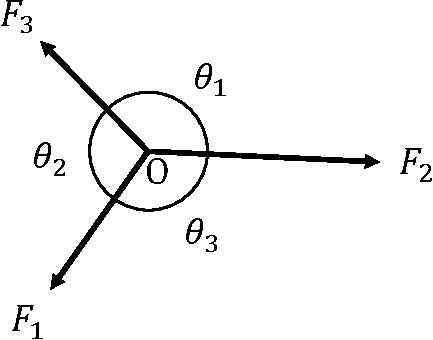
\includegraphics[width=4cm]{lami-s-theorem.pdf}
  \caption{3力の釣合いとラミの定理}
  \label{fig:lami-s-theorem}
\end{figure}

% ここまで編集してください

\end{document}
